\chapter{Introduction to networks}

\textbf{Definition:} A \textit{graph} $G$ is a pair $(V, E)$, where $V$ is a set of vertices (or nodes), and $E$ is a set of edges, where each edge is a pair of vertices $(u, v) \in V \times V$. 
\begin{itemize}
 \item The vertices are said to be adjacent if they are endpoints of an edge. 
 \item The set of all edges incident to a vertex $v$ is called the \textit{neighborhood} of $v$, denoted by $\partial v$.
\end{itemize}
 

The \textit{adjacency matrix} $A_G$ of a graph $G$ is:
\begin{itemize}
 \item a square matrix of size $n \times n$, where $n = |V|$,
 \item if $(u,v)\in E$, then $A_G(u,v) = 1 $ 
 \item else $A_G(u,v) = 0 $
\end{itemize}


Consider the graph $G = (V, E)$, where $V = \{1,2,3,4\}$ and \[E = \{(1,2),(1,3),(2,3),(3,4)\}\]. The graph $G$ and its adjacency matrix $A_G$ are shown below:

\[
G = 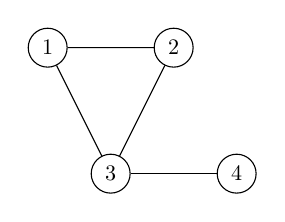
\begin{tikzpicture}[scale=0.8, transform shape]
    \node[shape=circle,draw=black] (1) at (0,2) {1};
    \node[shape=circle,draw=black] (2) at (2,2) {2};
    \node[shape=circle,draw=black] (3) at (1,0) {3};
    \node[shape=circle,draw=black] (4) at (3,0) {4};
    \draw[-] (1) -- (2);
    \draw[-] (1) -- (3);
    \draw[-] (2) -- (3);
    \draw[-] (3) -- (4);
\end{tikzpicture} \qquad A_G = \begin{bmatrix}
0 & 1 & 1 & 0 \\
1 & 0 & 1 & 0 \\
1 & 1 & 0 & 1 \\
0 & 0 & 1 & 0
\end{bmatrix}
\]


%In the adjacency matrix $A_G$, the entry $A_G(i,j)$ is 1 if there is an edge between vertices $i$ and $j$ in the graph $G$, and 0 otherwise. For example, $A_G(1,2) = 1$, since there is an edge between vertices 1 and 2 in the graph $G$.

\textbf{Degree of a Node:} The \textit{degree} of a node $v$ in a graph $G = (V,E)$ is the number of edges incident to $v$, i.e., the number of neighbors of $v$. The degree of $v$ is denoted by $deg(v)$. In a directed graph, the degree of a node is the sum of its in-degree (number of incoming edges) and out-degree (number of outgoing edges).

\textbf{Neighborhood of a Node:} The \textit{neighborhood} of a node $v$ in a graph $G = (V,E)$ is the set of all nodes that are adjacent to $v$, i.e., the set of all neighbors of $v$. The neighborhood of $v$ is denoted by $\partial_v$.

For example, in the previous graph, the degree of node 1 is 2, since it has 2 neighbors (nodes 2 and 3), i.e., $deg(1) = 2$. Similarly, the degree of node 2 is 2 and the degree of node 3 is 3. The degree of node 4 is 1, since it has only 1 neighbor (node 3).

The neighborhood of node 1 is $\partial_1 = \{2, 3\}$, since nodes 2 and 3 are adjacent to node 1. Similarly, the neighborhood of node 2 is $\partial_2 = \{1, 3\}$, the neighborhood of node 3 is $\partial_3 = \{1, 2, 4\}$, and the neighborhood of node 4 is $\partial_4 = \{3\}$.

The adjacency matrix can be used to compute various properties of the graph, such as the number of paths of a certain length between two vertices, the number of cycles of a certain length in the graph, and many others.


\textbf{Paths:} A \textit{path} in a graph $G=(V,E)$ is a sequence of distinct vertices $v_1, v_2, \ldots, v_k$ such that $(v_i, v_{i+1}) \in E$ for $i=1,2,\ldots,k-1$. The length of the path is $k-1$, and it is denoted by $|P|$. A path is said to be \textit{simple} if all its vertices are distinct.

\textbf{Cycles:} A \textit{cycle} in a graph $G=(V,E)$ is a simple path $v_1, v_2, \ldots, v_k$ such that $(v_k, v_1) \in E$. The length of the cycle is $k$, and it is denoted by $|C|$.

\textbf{Adjacency Matrix and Paths:} The adjacency matrix $A_G$ of a graph $G$ can be used to compute the number of paths between two nodes $u$ and $v$ in the graph. The entry $(A_G)^n(u,v)$ gives the number of paths of length $n$ between nodes $u$ and $v$. Specifically, the $(u,v)$ entry of $A_G^n$ gives the number of paths of length $n$ from node $u$ to node $v$.

To see why this is true, consider the $(u,v)$ entry of $A_G^2$. This entry is given by $(A_G^2)_{u,v} = \sum_{w \in V} A_G(u,w) A_G(w,v)$, which counts the number of paths of length 2 from $u$ to $v$ by summing over all possible intermediate nodes $w$. By induction, we can show that $(A_G)^n(u,v)$ counts the number of paths of length $n$ between nodes $u$ and $v$.

In the previous graph, to compute the number of paths of length 2 between nodes 1 and 4, we can compute $(A_G)^2(1,4)$, which is equal to $[(A_G)^2]_{1,4} = A_G(1,2)A_G(2,3) + A_G(1,3)A_G(3,4) = 1 \cdot 1 + 1 \cdot 1 = 2$. Therefore, there are two paths of length 2 between nodes 1 and 4 in the graph $G$.

The adjacency matrix of a graph $G$ can also be used to compute the number of cycles of a certain length $k$ in the graph. Specifically, the $(i,j)$ entry of the matrix $A_G^k$ gives the number of cycles of length $k$ that contain the edge $(i,j)$.

To see why this is true, consider the $(i,j)$ entry of $A_G^k$. This entry is given by $(A_G^k)_{i,j} = \sum_{w_1, w_2, \ldots, w_{k-1}} A_G(i,w_1) A_G(w_1,w_2) \cdots A_G(w_{k-1},j)$, which counts the number of paths of length $k$ from $i$ to $j$ by summing over all possible intermediate nodes $w_1, w_2, \ldots, w_{k-1}$. If the edge $(i,j)$ is part of a cycle of length $k$, then we have $w_1, w_2, \ldots, w_{k-1} \neq i,j$ and the last term $A_G(w_{k-1},j)$ in the sum will be equal to 1 (since $(w_{k-1}, j)$ is an edge in the cycle), while all other terms in the sum will be nonzero. Therefore, the $(i,j)$ entry of $A_G^k$ will count the number of cycles of length $k$ that contain the edge $(i,j)$.

For example, let's consider the following graph $G$:

\[
G = 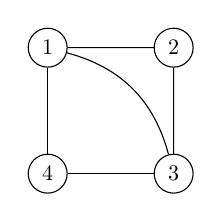
\begin{tikzpicture}[scale=0.8, transform shape]
    \node[shape=circle,draw=black] (1) at (0,2) {1};
    \node[shape=circle,draw=black] (2) at (2,2) {2};
    \node[shape=circle,draw=black] (3) at (2,0) {3};
    \node[shape=circle,draw=black] (4) at (0,0) {4};
    \draw[-] (1) -- (2);
    \draw[-] (2) -- (3);
    \draw[-] (3) -- (4);
    \draw[-] (4) -- (1);
    \draw[-] (1) to [bend left=30] (3);
\end{tikzpicture}
\]

The adjacency matrix of $G$ is:

\[
A_G = \begin{bmatrix}
0 & 1 & 0 & 1 \\
1 & 0 & 1 & 0 \\
0 & 1 & 0 & 1 \\
1 & 0 & 1 & 0
\end{bmatrix}
\]

To compute the number of cycles of length 3 in the graph $G$, we can compute the matrix $A_G^3$ and count the number of entries that are nonzero. Since we are interested in cycles of length 3, we only need to consider the entries of $A_G^3$ that correspond to edges in the graph $G$. For example, the entry $(1,2)$ of $A_G^3$ gives the number of cycles of length 3 that contain the edge $(1,2)$. We have:

\begin{align*}
(A_G^3)_{1,2} &= \sum_{w_1, w_2} A_G(1,w_1) A_G(w_1,w_2) A_G(w_2,2) \\
&= A_G(1,4) A_G(4,3) A_G(3,2) \\
&= 1 \cdot 1 \cdot 1 \\
&= 1
\end{align*}

Therefore, there is exactly one cycle of length 3 in the graph $G$ that contains the edge $(1,2)$. Similarly, we can compute the other entries of $A_G^3$ to count the number of cycles of length 3 that contain the other edges in the graph. In this case, we find that there are three cycles of length 3 in the graph $G$.

\section{Directed graphs}

No problem, here's a directed version of the graph you requested:

\[
G = 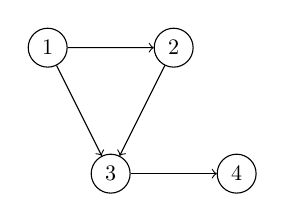
\begin{tikzpicture}[->, scale=0.8, transform shape]
\node[shape=circle,draw=black] (1) at (0,2) {1};
\node[shape=circle,draw=black] (2) at (2,2) {2};
\node[shape=circle,draw=black] (3) at (1,0) {3};
\node[shape=circle,draw=black] (4) at (3,0) {4};
\draw[->] (1) -- (2);
\draw[->] (1) -- (3);
\draw[->] (2) -- (3);
\draw[->] (3) -- (4);
\end{tikzpicture}
\]

The adjacency matrix of $G$ is:

\[
A_G = \begin{bmatrix}
0 & 1 & 1 & 0 \\
0 & 0 & 1 & 0 \\
0 & 0 & 0 & 1 \\
0 & 0 & 0 & 0
\end{bmatrix}
\]

To compute the in-degree and out-degree of each vertex in the graph $G$, we can sum the entries of the corresponding rows and columns in the adjacency matrix. We have:

\begin{itemize}
  \item Vertex 1: in-degree = 0, out-degree = 2
  \item Vertex 2: in-degree = 1, out-degree = 1
  \item Vertex 3: in-degree = 2, out-degree = 1
  \item Vertex 4: in-degree = 1, out-degree = 0
\end{itemize}

In this case, vertex 1 and vertex 4 are sources and sink, respectively.

\section{Wheigted graphs}

A weighted graph is a graph where each edge has a numerical value associated with it, called a weight. The weight often represents some sort of cost, distance, or importance associated with traversing the edge.

In mathematical terms, a weighted graph is represented by a graph $G = (V, E, w)$, where $V$ is the set of vertices (nodes), $E$ is the set of edges, and $w :  E \rightarrow \mathbb{R}$ is a function that assigns a weight to each edge.

\[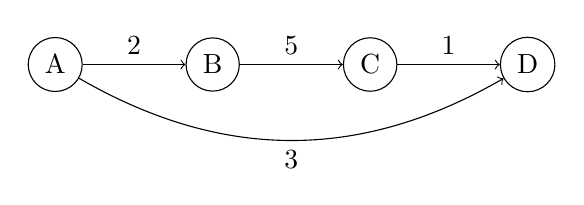
\begin{tikzpicture}
  \node[circle, draw] (A) at (0,0) {A};
  \node[circle, draw] (B) at (2,0) {B};
  \node[circle, draw] (C) at (4,0) {C};
  \node[circle, draw] (D) at (6,0) {D};
  \draw[->] (A) -- node[above] {2} (B);
  \draw[->] (B) -- node[above] {5} (C);
  \draw[->] (C) -- node[above] {1} (D);
  \draw[->] (A) to[bend right] node[below] {3} (D);
\end{tikzpicture}\]
In this example, we define a weighted graph with four nodes (A, B, C, and D) and four edges with weights (2, 5, 1, and 3). 
In this graph, the weights on the edges represent the cost or distance associated with traversing the edge. For example, to get from node A to node D, we could either take the edge with weight 2 and the edge with weight 1, or we could take the edge with weight 3. The choice of which path to take would depend on the specific application of the graph.

\section{Graphs properties}

1. {\bf Connected vs Disconnected Graphs}: A connected graph is a graph where there is a path between any two vertices in the graph. A disconnected graph is a graph that is not connected, meaning that there are at least two vertices that are not connected by a path. For example, the following graph is connected:

\[
G = 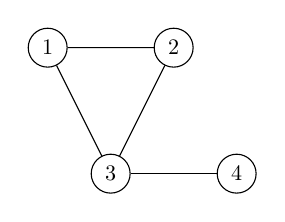
\begin{tikzpicture}[scale=0.8, transform shape]
\node[shape=circle,draw=black] (1) at (0,2) {1};
\node[shape=circle,draw=black] (2) at (2,2) {2};
\node[shape=circle,draw=black] (3) at (1,0) {3};
\node[shape=circle,draw=black] (4) at (3,0) {4};
\draw[-] (1) -- (2);
\draw[-] (1) -- (3);
\draw[-] (2) -- (3);
\draw[-] (3) -- (4);
\end{tikzpicture}
\]

while the following graph is disconnected:

\[
G = 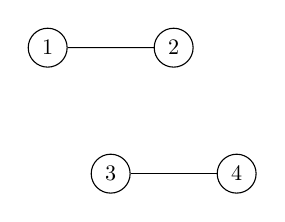
\begin{tikzpicture}[scale=0.8, transform shape]
\node[shape=circle,draw=black] (1) at (0,2) {1};
\node[shape=circle,draw=black] (2) at (2,2) {2};
\node[shape=circle,draw=black] (3) at (1,0) {3};
\node[shape=circle,draw=black] (4) at (3,0) {4};
\draw[-] (1) -- (2);
\draw[-] (3) -- (4);
\end{tikzpicture}
\]

2. {\bf Regular vs Non-Regular Graphs}: A regular graph is a graph where all vertices have the same degree, meaning that each vertex has the same number of neighbors. A non-regular graph is a graph where the degrees of the vertices are not all the same. For example, the following graph is regular:

\[
G = 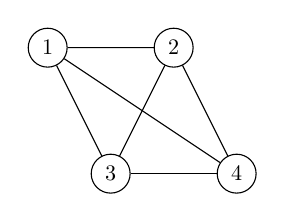
\begin{tikzpicture}[scale=0.8, transform shape]
\node[shape=circle,draw=black] (1) at (0,2) {1};
\node[shape=circle,draw=black] (2) at (2,2) {2};
\node[shape=circle,draw=black] (3) at (1,0) {3};
\node[shape=circle,draw=black] (4) at (3,0) {4};
\draw[-] (1) -- (2);
\draw[-] (1) -- (3);
\draw[-] (1) -- (4);
\draw[-] (2) -- (3);
\draw[-] (2) -- (4);
\draw[-] (3) -- (4);
\end{tikzpicture}
\]

while the following graph is non-regular:

\[
G = 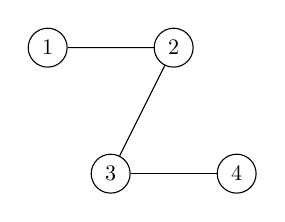
\begin{tikzpicture}[scale=0.8, transform shape]
\node[shape=circle,draw=black] (1) at (0,2) {1};
\node[shape=circle,draw=black] (2) at (2,2) {2};
\node[shape=circle,draw=black] (3) at (1,0) {3};
\node[shape=circle,draw=black] (4) at (3,0) {4};
\draw[-] (1) -- (2);
\draw[-] (2) -- (3);
\draw[-] (3) -- (4);
\end{tikzpicture}
\]

3. {\bf Planar vs Non-Planar Graphs:} A planar graph is a graph that can be drawn on a plane without any edges crossing. A non-planar graph is a graph that cannot be drawn on a plane without any edges crossing. For example, the following previous non regular graph is planar, while the following graph is non-planar:
\[
G = 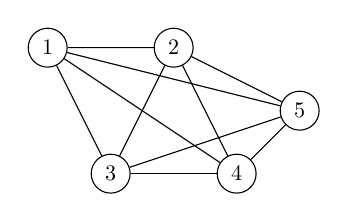
\begin{tikzpicture}[scale=0.8, transform shape]
\node[shape=circle,draw=black] (1) at (0,2) {1};
\node[shape=circle,draw=black] (2) at (2,2) {2};
\node[shape=circle,draw=black] (3) at (1,0) {3};
\node[shape=circle,draw=black] (4) at (3,0) {4};
\node[shape=circle,draw=black] (5) at (4,1) {5};
\draw[-] (1) -- (2);
\draw[-] (1) -- (3);
\draw[-] (2) -- (3);
\draw[-] (3) -- (4);
\draw[-] (4) -- (1);
\draw[-] (4) -- (5);
\draw[-] (4) -- (2);
\draw[-] (1) -- (5);
\draw[-] (2) -- (5);
\draw[-] (3) -- (5);
\end{tikzpicture}
\]
Less trivially, the previous example of a regular graph is also planar, although it doesn't seem so. Check that moving node 4 to the inside of the triangle created by the other three nodes, you can actually paint it without crossing lines.

4.{\bf Bipartite Graphs}: A bipartite graph is a graph where the vertices can be divided into two sets such that there is no edge between vertices in the same set. The previous example of a non-planar graph, is also a non-bipartite graph. On the contrary, the following graph is bipartite with sets $\{1,2\}$ and $\{3,4\}$:
\[
 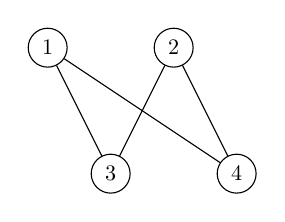
\begin{tikzpicture}[scale=0.8, transform shape]
\node[shape=circle,draw=black] (1) at (0,2) {1};
\node[shape=circle,draw=black] (2) at (2,2) {2};
\node[shape=circle,draw=black] (3) at (1,0) {3};
\node[shape=circle,draw=black] (4) at (3,0) {4};
\draw[-] (1) -- (3);
\draw[-] (1) -- (4);
\draw[-] (2) -- (3);
\draw[-] (2) -- (4);
\end{tikzpicture}
\]

5. {\bf Trees:} A tree is a connected graph with no cycles, meaning that there is exactly one path between any two vertices in the graph. For example, the following graph is a tree:
\[
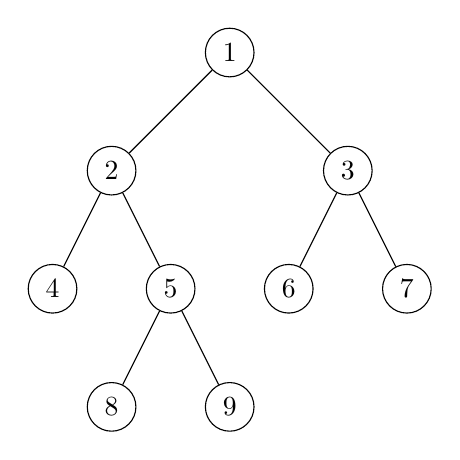
\begin{tikzpicture}[level distance=1.5cm,
  level 1/.style={sibling distance=3cm},
  level 2/.style={sibling distance=1.5cm}]
  \node[circle,draw](1){$1$}
    child{node[circle,draw](2){$2$}
      child{node[circle,draw](4){$4$}}
      child{node[circle,draw](5){$5$}
        child{node[circle,draw](8){$8$}}
        child{node[circle,draw](9){$9$}}
      }
    }
    child{node[circle,draw](3){$3$}
      child{node[circle,draw](6){$6$}}
      child{node[circle,draw](7){$7$}}
    };
\end{tikzpicture}\]

Trees are important in many applications, such as in computer science where they are used to represent hierarchical structures like file systems or organization charts.

\section{Graph metrics}

Centrality measures are used to quantify the importance of individual nodes in a network. There are several types of centrality measures, including degree centrality, betweenness centrality, and eigenvector centrality. Degree centrality is based on the number of edges incident to a node, while betweenness centrality measures the fraction of shortest paths in the network that pass through a node. Eigenvector centrality takes into account the centrality of a node's neighbors, and assigns higher centrality to nodes that are connected to other highly central nodes.

\subsection{Density of a graph and mean degree}
For a graph $G(V,E)$, density is defined as
\[ D = \frac {|E|}{|V|}\]
Graphs with $D \ll 1$ are named sparse.

The average degree of a graph is given by
\[ \langle k \rangle  = \sum_k k P(k) = \frac{2 |E|}{|V|} = 2 D\]

Second moment (variance):
\[ \sigma_k^2 = \langle k^2 \rangle -\langle k \rangle^2  = \sum_k (k -\langle k \rangle)^2 P(k)\]
A graph is called heterogeneous if 
\[\frac {\sigma_k} {\langle k \rangle} \gg 1\]


\subsection{Diameter, radius, eccentricity}

The eccentricity $\epsilon(v)$ of a vertex $v$ is the greatest distance between v and any other vertex; in symbols,
\[   {\displaystyle \epsilon (v)=\max_{u\in V}d(v,u).}
\]
It can be thought of as how far a node is from the node most distant from it in the graph.

The radius r of a graph is the minimum eccentricity of any vertex or, in symbols,
\begin{eqnarray*}
    r &=& \min_{ v \in V} \epsilon (v) = \min_{v \in V} \max_{ u \in V} d ( v , u ) 
\end{eqnarray*}
The diameter d of a graph is the maximum eccentricity of any vertex in the graph. That is, d is the greatest distance between any pair of vertices or, alternatively,
\[
    d = \max\limits_{\left(v \in V \right)}  \epsilon ( v ) = \max\limits_{\left(v \in V \right)}   \max\limits_{\left( u \in V \right)}    d ( v , u ) 
\]
To find the diameter of a graph, first find the shortest path between each pair of vertices. The greatest length of any of these paths is the diameter of the graph.

A central vertex in a graph of radius r is one whose eccentricity is r—that is, a vertex whose distance from its furthest vertex is equal to the radius, equivalently, a vertex v such that $\epsilon(v) = r$.

A peripheral vertex in a graph of diameter d is one whose eccentricity is d—that is, a vertex whose distance from its furthest vertex is equal to the diameter. Formally, v is peripheral if $\epsilon(v) = d$.

\subsection{Jordan centrality measure}

The center (or Jordan center) of a graph is the set of all vertices of minimum eccentricity, that is, the set of all vertices $u$ where the greatest distance $d(u,v)$ to other vertices $v$ is minimal. Equivalently, it is the set of vertices with eccentricity equal to the graph's radius:
\[ \{ v_1,\ldots,v_n \} | \forall_{i\in 1\ldots n} \epsilon (v_i) = r \]
Thus vertices in the center (central points) minimize the maximal distance from other points in the graph. 

\subsection{Degree centrality}
Degree centrality is a measure of the importance of a node in a network based on the number of edges incident to the node. Mathematically, the degree centrality $C_d$ of a node $i$ in a network $G$ is defined as:
\begin{equation}
    C_d(i) = \frac{k_i}{n-1},
\end{equation}
where $k_i$ is the number of edges incident to node $i$, and $n$ is the total number of nodes in the network. The degree centrality ranges from 0 to 1, with higher values indicating greater importance.

Degree centrality is a simple and intuitive measure of node importance, and is commonly used in social network analysis, biological networks, and other types of networks. However, it does not take into account the importance of the nodes to which a node is connected, and may not be the most appropriate measure for all types of networks.


\subsection{Betweenness}

Betweenness centrality is a measure of the importance of a node in a network based on the number of shortest paths that pass through the node. Mathematically, the betweenness centrality $C_b$ of a node $i$ in a network $G$ is defined as:

\begin{equation}
    C_b(i) = \sum_{s \neq i \neq t} \frac{\sigma_{st}(i)}{\sigma_{st}},
\end{equation}
where $\sigma_{st}$ is the total number of shortest paths between nodes $s$ and $t$, and $\sigma_{st}(i)$ is the number of shortest paths that pass through node $i$. The sum is taken over all pairs of nodes $s$ and $t$ that are not equal to node $i$. 

The betweenness centrality ranges from 0 to 1, with higher values indicating greater importance. Nodes with high betweenness centrality are important for maintaining communication and facilitating the flow of information in the network.

The calculation of betweenness centrality can be computationally intensive for large networks, but efficient algorithms have been developed to approximate the betweenness centrality of nodes in large networks.

\subsection{Modularity}

Modularity is a measure of the division of a network into dense clusters or communities. So the value of the modularity is not associated to a graph by it self, but to a graph and a partition of it's nodes into different communities. Communities are specified by numbers $s_i \i \{1\ldots,k\}$, such that  $s_i$ is the number of the community that node $i$ belongs to.


Mathematically, the modularity $Q$ of a network $G$ with a partition $s$ of nodes into $k$ communities is defined as:
\begin{equation}
    Q = \frac{1}{2m} \sum_{i,j} \left( A_{ij} - \frac{k_i k_j}{2m} \right) \delta(s_i, s_j),
\end{equation}
where $A_{ij}$ is the weight of the edge between nodes $i$ and $j$, $k_i$ and $k_j$ are the degrees of nodes $i$ and $j$, respectively, $m$ is the total weight of edges in the network, and $\delta(s_i, s_j)$ is the Kronecker delta function that equals 1 if nodes $i$ and $j$ belong to the same community, and 0 otherwise. 

The modularity ranges from -1 to 1, with higher values indicating a more modular network structure. A modularity of 0 indicates that the partition of nodes into communities is no better than chance. A modularity near 1 (homophily) indicate that nodes tend to connect to others of the same community, rather than a different one. Modularity near $-1$ indicates the opposite (paraphily).

The modularity can be used to evaluate the goodness of fit of different community detection algorithms and to compare the modular structure of different networks.

The calculation of modularity can be computationally intensive for large networks, but efficient algorithms have been developed to approximate the modularity of networks with millions of nodes and edges.

\subsection{Clustering}

The clustering coefficient is a measure of the degree to which nodes in a network tend to cluster together. It is defined as the fraction of the node's neighbors that are also neighbors of each other. Mathematically, the clustering coefficient $C_i$ of a node $i$ in a network $G$ is defined as:
\begin{equation}
    C_i = \frac{2e_i}{k_i (k_i - 1)},
\end{equation}
where $e_i$ is the number of edges between the neighbors of node $i$, and $k_i$ is the degree of node $i$, i.e., the number of edges incident to node $i$. The clustering coefficient ranges from 0 to 1, with higher values indicating that nodes in the network tend to form tightly interconnected clusters or communities. A low clustering coefficient indicates a more random and dispersed network structure.

The average clustering coefficient $C$ of a network $G$ is defined as the average of the clustering coefficients of all nodes in the network:
\begin{equation}
    C = \frac{1}{n} \sum_{i=1}^n C_i,
\end{equation}
where $n$ is the total number of nodes in the network.

The clustering coefficient is a useful tool for characterizing the local structure of a network, and can be used to identify nodes that are part of tightly interconnected clusters or communities. However, it does not provide information about the global structure of the network or the connections between clusters.

These concepts are important tools for analyzing the structure and function of complex networks, and have applications in a wide range of fields, including social network analysis, biological networks, and transportation networks.

\section{Assortativity}



\section{Laplacian of a graph}

The Laplacian of a graph is a matrix that encodes important information about the structure of the graph. The Laplacian is defined as the difference between the degree matrix and the adjacency matrix of the graph. The degree matrix is a diagonal matrix whose entries are the degrees of each vertex, while the adjacency matrix is a binary matrix that indicates which pairs of vertices are connected by an edge.

Given a graph $G$ with $n$ vertices, the Laplacian matrix $L$ is defined as:

$$L = D - A$$

where $D$ is the degree matrix and $A$ is the adjacency matrix of $G$. The Laplacian matrix is an $n \times n$ symmetric positive semidefinite matrix, and it has several important properties that make it useful in the study of graph theory and related fields.

Here's an example of how to compute the Laplacian matrix for a small graph with 4 vertices:

\[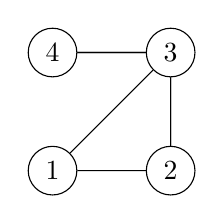
\begin{tikzpicture}[scale=1.5]
  \node[circle,draw] (1) at (0,0) {1};
  \node[circle,draw] (2) at (1,0) {2};
  \node[circle,draw] (3) at (1,1) {3};
  \node[circle,draw] (4) at (0,1) {4};
  \draw (1) -- (2) -- (3) -- (4);
  \draw (1) -- (3);
  \draw (2) -- (3);
  \draw (3) -- (4);
\end{tikzpicture} \]

The adjacency matrix $A$ and degree matrix $D$ for this graph is:
$$A = \begin{bmatrix}0 & 1 & 1 & 0 \\ 1 & 0 & 1 & 0 \\ 1 & 1 & 0 & 1 \\ 0 & 0 & 1 & 0\end{bmatrix} \qquad 
D = \begin{bmatrix}2 & 0 & 0 & 0 \\ 0 & 2 & 0 & 0 \\ 0 & 0 & 3 & 0 \\ 0 & 0 & 0 & 1\end{bmatrix}$$

The Laplacian matrix $L$ is:

$$L = D - A = \begin{bmatrix}2 & 0 & 0 & 0 \\ 0 & 2 & 0 & 0 \\ 0 & 0 & 3 & 0 \\ 0 & 0 & 0 & 1\end{bmatrix} - \begin{bmatrix}0 & 1 & 1 & 0 \\ 1 & 0 & 1 & 0 \\ 1 & 1 & 0 & 1 \\ 0 & 0 & 1 & 0\end{bmatrix} = \begin{bmatrix}2 & -1 & -1 & 0 \\ -1 & 2 & -1 & 0 \\ -1 & -1 & 3 & -1 \\ 0 & 0 & -1 & 1\end{bmatrix}$$

The Laplacian of the graph encodes important information about the connectivity and structure of the graph. For example, the number of connected components of the graph is equal to the number of eigenvectors of the Laplacian with eigenvalue 0. The Laplacian also plays an important role in spectral graph theory, where it is used to analyze the spectral properties of graphs and to design graph clustering algorithms.

\section{Networks for benchmarking}

1. Zachary's karate club network: This is a social network of a karate club that was studied by Zachary in 1977. The network consists of 34 nodes representing members of the club and 78 edges representing friendships between members. It is often used as a benchmark for community detection algorithms.

2. Erdős-Rényi random network: This is a random graph model proposed by Erdős and Rényi in 1959. In this model, a graph is generated by connecting nodes with a certain probability p. Erdős-Rényi random networks are often used as a benchmark for studying properties of random graphs.

3. Barabási-Albert preferential attachment network: This is a random graph model proposed by Barabási and Albert in 1999. In this model, a graph is generated by starting with a small number of nodes and adding new nodes one at a time, with each new node preferentially attaching to existing nodes with higher degree. Barabási-Albert networks are often used as a benchmark for studying properties of scale-free networks.

4. Les Miserables co-occurrence network: This is a network of co-occurrences of characters in the novel Les Miserables by Victor Hugo. The network consists of 77 nodes representing characters and 254 edges representing co-occurrences in the same chapter. It is often used as a benchmark for community detection algorithms.

5. Power grid network: This is a network of the power grid in the western United States. The network consists of 4,941 nodes representing power stations and 6,594 edges representing power lines. It is often used as a benchmark for studying properties of real-world networks.

6. The Southern Women graph is a social network graph that represents the social interactions between women in a Southern US social club in the 1930s. The graph is an undirected graph with 32 nodes (women) and 89 edges (social interactions).

Each node in the graph represents a woman, and an edge between two nodes indicates that the corresponding women interacted socially at the club. The weight of each edge represents the number of social events at which the two women interacted.

\subsection{Random graphs}

Random graphs are mathematical models that are used to study the properties of graphs that arise from random processes. In a random graph, edges are created between nodes according to some probabilistic model, rather than being determined by some underlying structure or pattern.


Example. There are two possible regular graphs with 4 nodes and degree 2: the cycle graph $C_4$
\begin{center}
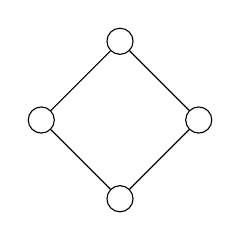
\begin{tikzpicture}
  \node[circle, draw] (A) at (0,0) {};
  \node[circle, draw] (B) at (1,1) {};
  \node[circle, draw] (C) at (2,0) {};
  \node[circle, draw] (D) at (1,-1) {};
  \draw (A) -- (B) -- (C) -- (D) -- (A);
\end{tikzpicture}
\end{center}
 and the disjoint union of two edges $K_2 \cup K_2$ :
\begin{center}
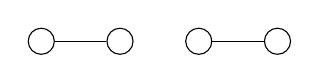
\begin{tikzpicture}
  \node[circle, draw] (A) at (0,0) {};
  \node[circle, draw] (B) at (1,0) {};
  \node[circle, draw] (C) at (2,0) {};
  \node[circle, draw] (D) at (3,0) {};
  \draw (A) -- (B);
  \draw (C) -- (D);
\end{tikzpicture}
\end{center}
These are the only two possible regular graphs with 4 nodes and degree 2, as any other arrangement would either have nodes of degree greater than 2 or have disconnected nodes. An algorithm that randomly produces one of these two graphs, produces random regular graphs.

There are many different models of random graphs, each with their own set of assumptions and properties. Some common models include:
\begin{itemize}
\item Erdős-Rényi model: A model where each edge is present with a fixed probability, independently of all other edges.
\item Watts-Strogatz model: A model where edges are rewired with a small probability, resulting in a graph with a high clustering coefficient but a short average path length.
\item Barabási-Albert model: A model where new nodes are added to the graph one at a time, and each new node is connected to existing nodes with a probability proportional to their degree.
\end{itemize}

\subsection{Random regular graphs}

Random regular graphs are graphs where each vertex has the same degree. The algorithm to generate a random regular graph with $n$ vertices and degree $k$ is as follows:

1. If $n$ is odd or $k$ is odd and $n$ is even, then no random regular graph exists. Otherwise, set $d = \frac{k}{2}$.
2. Create an empty graph $G$ with $n$ vertices.
3. For each vertex $v$, add an edge between $v$ and the $d$ vertices that appear next to it in a cyclic ordering of the vertices.
4. Shuffle the vertices randomly.
5. For each vertex $v$, rewire each of its $d$ edges to a randomly chosen vertex, subject to the constraints that the resulting graph remains $k$-regular and does not contain self-loops or multiple edges.

The resulting graph is a random $k$-regular graph on $n$ vertices.

\begin{algorithmic}[1]
\Require $n$: number of vertices, $k$: degree of each vertex
\State If $n$ is odd or $k$ is odd and $n$ is even, then no random regular graph exists.
\State Otherwise, set $d = \frac{k}{2}$.
\State Create an empty graph $G$ with $n$ vertices.
\For{$i = 1$ to $n$}
    \For{$j = 1$ to $d$}
        \State Add an edge between vertex $i$ and vertex $(i+j) \mod n$.
    \EndFor
\EndFor
\State Shuffle the vertices randomly.
\For{$i = 1$ to $n$}
    \For{$j = 1$ to $d$}
        \State Choose a random vertex $v$ that is not adjacent to vertex $i$.
        \State Remove the edge between vertex $i$ and some neighbor of $i$ that appears $j$ positions after $i$ in the cyclic ordering of vertices.
        \State Add an edge between vertex $i$ and vertex $v$.
    \EndFor
\EndFor
\State Output the resulting graph $G$.
\end{algorithmic}

\subsection{Erdos-Renyi model}
The Erdős-Rényi (ER) algorithm is a popular method for generating random graphs. Given a set of $n$ nodes and a probability $p$ of any two nodes being connected by an edge, the ER algorithm generates a random graph by considering each possible edge and including it with probability $p$.

The ER algorithm can be implemented as follows:
\begin{enumerate}
\item Start with an empty graph $G$ with $n$ nodes.
\item For each pair of nodes $i$ and $j$ (excluding self-loops), add an edge between them with probability $p$. This can be done by generating a random number $r$ between 0 and 1 for each pair of nodes, and adding an edge if $r \leq p$.
\item Output the resulting graph $G$.
\end{enumerate}

\begin{algorithmic}[1]
\Require $n$: number of nodes, $p$: probability of an edge between any pair of nodes
\State Create an empty graph $G$ with $n$ nodes.
\For{$i = 1$ to $n-1$}
    \For{$j = i+1$ to $n$}
        \State Generate a random number $r$ between 0 and 1.
        \If{$r \leq p$}
            \State Add an edge between nodes $i$ and $j$.
        \EndIf
    \EndFor
\EndFor
\State Output the resulting graph $G$.
\end{algorithmic}

The ER algorithm generates a random graph with an expected number of edges equal to $p \cdot \binom{n}{2}$, which is the number of possible edges in the graph multiplied by the probability of each edge being included. The resulting graph is typically sparse for small values of $p$ and becomes increasingly dense as $p$ approaches 1.

%The ER algorithm is a simple and effective way to generate random graphs with a given size and edge density, and it has been widely used in the study of graph theory and network science.

\subsection{Albert Barabasi graphs}

The Barabási-Albert (BA) algorithm is a popular method for generating scale-free graphs, which are graphs with a degree distribution that follows a power law. The BA algorithm generates a graph by starting with a small number of nodes and adding new nodes one at a time, each with a fixed number of edges attached to existing nodes.

The BA algorithm can be implemented as follows:

1. Start with a small graph $G$ with $m_0$ nodes, where $m_0$ is a parameter of the algorithm.
2. Add a new node $i$ to the graph, and connect it to $m$ existing nodes in the graph, where $m$ is a parameter of the algorithm.
3. The probability that node $i$ connects to node $j$ is proportional to the degree of node $j$ in the graph, i.e., nodes with higher degree are more likely to be connected to.
4. Repeat steps 2-3 until the desired number of nodes is reached.

\begin{algorithmic}[1]
\Require $m_0$: number of initial nodes, $m$: number of edges to attach to each new node, $n$: final number of nodes in the graph
\State Create an empty graph $G$ with $m_0$ nodes.
\State Create a list $L$ of nodes, where each node appears $m_0$ times in the list.
\For{$i = m_0$ to $n-1$}
    \State Create a new node $v_i$.
    \State Choose $m$ distinct nodes to connect $v_i$ to, sampled from $L$ with probability proportional to their degree.
    \State Add edges between $v_i$ and the chosen nodes.
    \State Add $m$ copies of $v_i$ to $L$.
\EndFor
\State Output the resulting graph $G$.
\end{algorithmic}

The resulting graph generated by the BA algorithm has a degree distribution that follows a power law, which means that a few nodes have a very high degree while most nodes have a low degree. This property is characteristic of many real-world networks, and it has important implications for the behavior of these networks.

The BA algorithm is a simple and elegant way to generate scale-free networks, and it has been widely used in the study of network science and related fields.

\section{Practical Python Class: networks}

\subsubsection*{Graph metrics in Les Miserables}



\section{Practical Homework}

\subsubsection*{Graph structure in written Chinese}

Take the list of Chinese words. Define a graph $G$ where each node is one Chinese character. Define a link between two nodes whenever there is at least one word with both characters.
\begin{enumerate}
 \item What is the degree distribution in $G$?
 \item Show examples of the characters with highest and smallest degree.
 \item Make a histogram of degree distribution? Is it heavytailed?
 \item Define the same graph, bot now directed, where direction is defined by the ordering of the characters in the words: $AB \Rightarrow (A\to B)$. Make the histogram of out-degree and in-degreen for the directed graph.
 \item Show examples of the charactes with highest out and in degrees.
 \item Make a hisogram of the out and in degrees.
 \item Define the unbalance, as the difference between out and in-degrees. Make a histogram of the unbalance.
 \item Show examples of characters with the high positive and negative unbalances. Is there a linguistic reason for this?
\end{enumerate}


\section{Percolation an epidemics}



